% -*- coding: utf-8; mode: latex; -*-

% beamer を使う
\documentclass[unicode,17pt]{beamer}

% LuaTeX-ja を使う
\usepackage{luatexja}
% 和文フォントは源ノ明朝 / 源ノ角ゴシックを使う、
% 複数のウェイトを使う、欧文フォントのファミリ指定と連動させる
\usepackage[sourcehan,deluxe,match]{luatexja-preset}

% 和文フォントの既定をゴシックに
\renewcommand{\kanjifamilydefault}{\gtdefault}

\usepackage{hologo}    % 各種 TeX ロゴ用
\usepackage{listings}  % ソースファイル表示用
\usepackage{tcolorbox} % 枠囲み用
\usepackage{multicol}  % 目次の 2 段組用
\usepackage[absolute,overlay]{textpos} % 座標指定用

% 数式フォント、欧文フォント設定
\usepackage{unicode-math}
\unimathsetup{math-style=ISO,bold-style=ISO}
\setmainfont{Libertinus Serif}
\setsansfont{Libertinus Sans}
\setmonofont{Source Code Pro}[Scale=MatchLowercase] %これだけ大きく見えるので
\setmathfont{Libertinus Math}

% スライドのデザイン
\useinnertheme{rounded}
\useoutertheme{infolines}
\usecolortheme[rgb={0.0,0.5,0.0}]{structure}
\usecolortheme{lily}
\usecolortheme{dolphin}
\setbeamertemplate{navigation symbols}{}

% スライドの背景画像
\usebackgroundtemplate{\includegraphics[height=\paperheight]%
  {none-background.png}}

% フォント関連
\usefonttheme{structurebold} % タイトル部を太字
\setbeamerfont{alerted text}{series=\bfseries} % Alertを太字
\setbeamerfont{section in toc}{series=\mdseries} % 目次は太字にしない
\setbeamerfont{date}{size=\small}  % 日付文字サイズ

% 目次に節番号をつける
\setbeamertemplate{section in toc}[sections numbered]

% hyperref 設定
\hypersetup{%
  pdftitle={Extract PDFmarkによるPDFファイルサイズ削減},% タイトル
  pdfsubject={TeXConf 2017 一般講演 発表資料},% サブタイトル
  pdfauthor={細田 真道},% 著者
  pdfkeywords={% キーワード
    Extract PDFmark, extractpdfmark, LilyPond, Texinfo, TeX, LaTeX,
    Ghostscript, PDF%
  },%
}

% listings 設定
\lstset{%
  basicstyle=\tiny\ttfamily,% フォント設定
  frame=none,% 枠を付けない(listings の枠線は隙間が空いてしまうので)
  lineskip=-0.6ex% 行間を詰める
}

\title[Extract PDFmark]{Extract PDFmarkによる \\ PDFファイルサイズ削減}
\author{細田 真道}
\institute[]{\url{http://www.trueroad.jp}}
\date[2017-10-14]{2017年10月14日}

\begin{document}

\begin{frame}
  \titlepage
  \begin{textblock*}{0.5\linewidth}(190pt,0pt)
    \begin{flushright}
      \tiny
      \href{https://texconf2017.tumblr.com/}%
           {TeXConf 2017} 一般講演 発表資料 \\
      Copyright (C) 2017 Masamichi Hosoda \\
      \href{https://creativecommons.org/licenses/by-sa/4.0/deed.ja}%
           {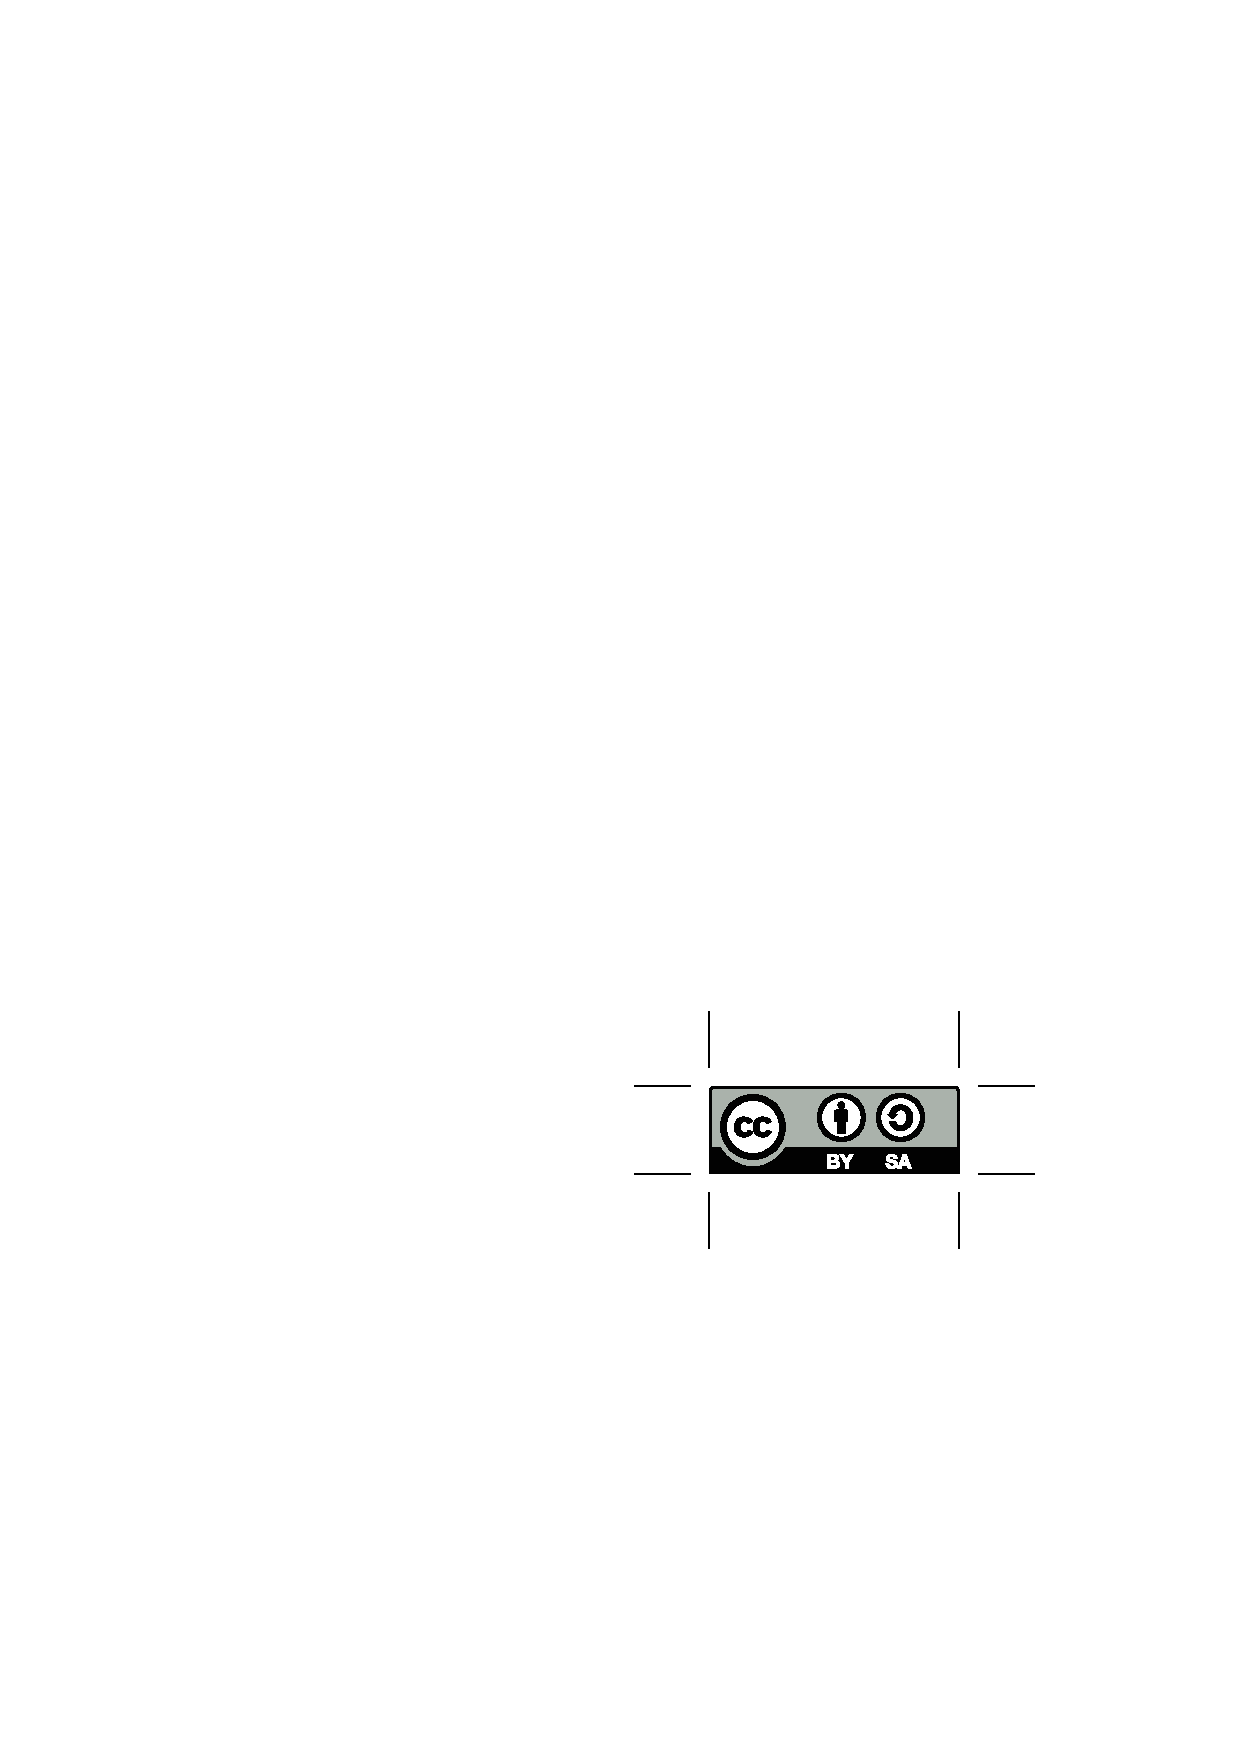
\includegraphics[height=3ex]{by-sa}}
    \end{flushright}
  \end{textblock*}
\end{frame}

\section*{自己紹介}
\begin{frame}\frametitle{自己紹介}
  \begin{itemize}
    \small
  \item 楽譜作成プログラムLilyPondコミッタ
    \begin{itemize}
    \item ビルドシステム、フォント、PDF等
    \end{itemize}
  \item GNU公式文書フォーマットTexinfoコミッタ
    \begin{itemize}
    \item \hologo{XeTeX}~/ \hologo{LuaTeX}、Unicode、日本語対応等
    \end{itemize}
  \item 第10回日本OSS奨励賞受賞
    \begin{itemize}
      \item LilyPond
    \end{itemize}
  \end{itemize}

  \begin{block}{}
    \begin{description}
      \footnotesize
      \setlength{\parskip}{0pt}
      \setlength{\itemsep}{0pt}
    \item[URL] \url{http://www.trueroad.jp}
    \item[GitHub] \href{https://github.com/trueroad/}%
      {\ttfamily trueroad}
    \item[Twitter] \href{https://twitter.com/trueroad_jp}%
      {\ttfamily @trueroad\_jp}
    \item[Facebook] \href{https://www.facebook.com/trueroad.jp}%
      {\ttfamily trueroad.jp}
    \item[GPG Key fingerprint]\mbox{}\\
      {\hspace{-3em} 49B8 ED79 B6A8 C46E 2F6D  ABB3 FCD0 C162 1E80 A02D}
    \end{description}
  \end{block}
\end{frame}

% Insert limited introduction here

\section*{目次}
\begin{frame}\frametitle{}\small\setlength{\columnseprule}{1pt}
  \begin{multicols}{2}%
    \tableofcontents
  \end{multicols}
\end{frame}

\section{はじめに}
\begin{frame}\frametitle{}
  \centering
  \usebeamerfont{frametitle}\usebeamercolor[fg]{frametitle}はじめに
\end{frame}

\begin{frame}\frametitle{はじめに}
  \begin{itemize}
  \item \TeX ~/ \LaTeX でPDFドキュメントを作成
    \begin{itemize}
    \item 図としてたくさんの小さなPDFを用意
    \item メインのPDFへ貼り付ける
    \end{itemize}
  \item 図PDFは同じフォントを使っていることが多い
  \end{itemize}
\end{frame}

\begin{frame}\frametitle{LilyPondの場合}
  \begin{itemize}
  \item マニュアルはTexinfo形式
    \begin{itemize}
    \item \hologo{XeTeX}で処理し、PDFを生成
    \end{itemize}
  \item 楽譜作成プログラムなので、、、
    \begin{itemize}
    \item マニュアルには楽譜の断片を多数含む
      \begin{itemize}
      \item LilyPondでPDFとして生成
      \item 図として貼り込む
      \end{itemize}
    \item もちろん同じフォントが多い
    \end{itemize}
  \end{itemize}
\end{frame}

\begin{frame}\frametitle{図PDFのフォント}
  \begin{itemize}
  \item 図PDFにフォントが埋め込まれていると、、、
    \begin{itemize}
    \item そのままメインPDFに埋め込まれる
    \end{itemize}
  \item 複数の図に同じフォントが埋め込まれていると
    \begin{itemize}
    \item メインPDFにフォントが重複して複数回埋め込まれる
    \end{itemize}
  \item ファイルサイズの増加につながる
  \end{itemize}
\end{frame}

\begin{frame}\frametitle{フォント重複防止}
  \begin{itemize}
  \item ファイルサイズを削減するには?
    \begin{itemize}
    \item 図PDF作成時に埋め込み方法を工夫
    \item メインPDFをGhostscriptで処理
    \end{itemize}
  \item しかし
    \begin{itemize}
    \item Ghostscriptで処理すると失われるものが
    \end{itemize}
  \end{itemize}
\end{frame}

\begin{frame}\frametitle{失われるもの}
  \begin{itemize}
  \item PDFページモード
    \begin{itemize}
    \item PDFを開いたときにどんな表示にするか
    \end{itemize}
  \item リンクの宛先名
    \begin{itemize}
    \item 外部から場所を指定したリンク
    \end{itemize}
  \item Extract PDFmark を使えば保持できます
  \end{itemize}
\end{frame}

\section{PDF}
\begin{frame}\frametitle{}
  \centering
  \usebeamerfont{frametitle}\usebeamercolor[fg]{frametitle}PDF
\end{frame}

\begin{frame}\frametitle{PDF}
  \begin{itemize}
  \item PDFの機能
    \begin{itemize}
    \item しおり
      \begin{itemize}
      \item ブックマーク、アウトライン、とも
      \end{itemize}
    \item ページモード
    \item ハイパーリンク
    \item フォント
    \end{itemize}
  \end{itemize}
\end{frame}

\subsection{しおり}
\begin{frame}\frametitle{しおり}
  \begin{itemize}
  \item 文書構造をツリー状に表示
    \begin{itemize}
    \item 章・節など
    \end{itemize}
  \item 目的の部分へ簡単にジャンプできる
    \begin{center}
      ここ→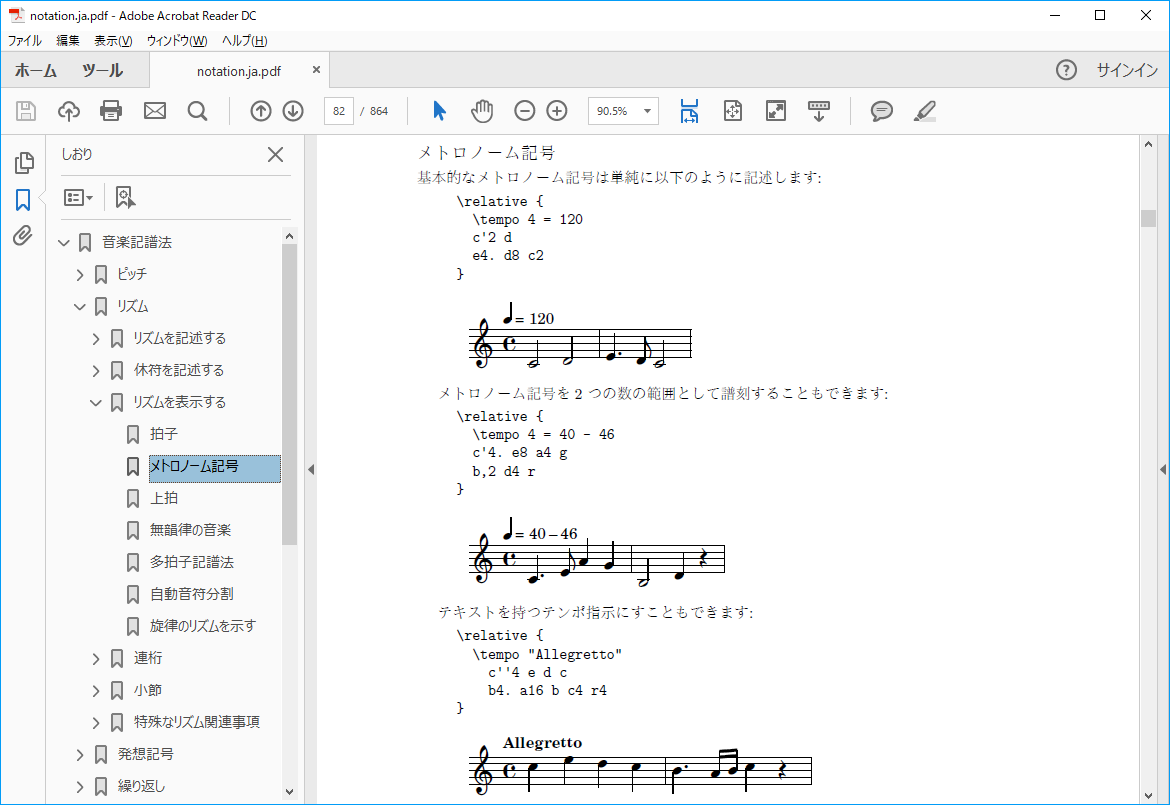
\includegraphics[width=0.7\linewidth]{notation-ja-capture.png}
    \end{center}
  \end{itemize}
\end{frame}

\subsection{ページモード}
\begin{frame}\frametitle{ページモード}
  \begin{itemize}
  \item ページモードを指定しておくと
    \begin{itemize}
    \item PDFを開いたとき、\\
      最初からしおりが表示される、など
    \end{itemize}
  \end{itemize}
\end{frame}

\subsection{ハイパーリンク}
\begin{frame}\frametitle{ハイパーリンク}
  \begin{itemize}
  \item リンクする
    \begin{itemize}
    \item URL
    \item 同じPDF内のどこか
    \item 他のPDFのどこか、など
    \end{itemize}
  \item リンクされる
    \begin{itemize}
    \item 宛先名(named destination)を設定
      \begin{itemize}
      \item 名前と場所を指定
      \item 名前に設定された場所へジャンプできる
      \end{itemize}
    \item PDF外部から名前を指定してリンク
      \begin{itemize}
      \item PDF相互間
      \item HTMLからのリンク、など
      \end{itemize}
    \end{itemize}
  \end{itemize}
\end{frame}

\subsection{フォント}
\begin{frame}\frametitle{フォント}
  \begin{itemize}
  \item フォントが無い環境でも正しく表示
  \item 埋め込み
    \begin{itemize}
    \item フルセット(非サブセット)埋め込み
      \begin{itemize}
      \item フォントを丸々フルセットで埋め込む
      \item ファイルサイズが大きくなる
      \end{itemize}
    \item サブセット埋め込み
      \begin{itemize}
      \item 使用しているグリフのみ埋め込む
      \item ファイルサイズを抑え正しく表示可
      \end{itemize}
    \item 非埋め込み
      \begin{itemize}
      \item フォントを埋め込まない
      \item ファイルサイズは最小
      \item 正しく表示できないことがある
      \end{itemize}
    \end{itemize}
  \end{itemize}
\end{frame}

\section{LilyPond}
\begin{frame}\frametitle{}
  \centering
  \usebeamerfont{frametitle}\usebeamercolor[fg]{frametitle}LilyPond
\end{frame}

\begin{frame}\frametitle{LilyPond}
  \begin{itemize}
  \item ソースファイルをコンパイル
  \end{itemize}
  \centering
  \tcbox[left=0mm,right=0mm,top=0mm,bottom=0mm]%
        {\lstinputlisting[linewidth=0.9\linewidth]{la_primavera-core.ly}}
  \begin{itemize}
  \item 楽譜のPDFなど生成
  \end{itemize}
  \centering
  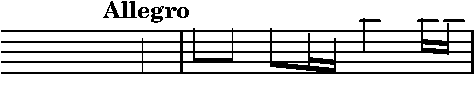
\includegraphics[width=0.7\linewidth]{la_primavera.pdf}
\end{frame}

\section{Texinfo}
\begin{frame}\frametitle{}
  \centering
  \usebeamerfont{frametitle}\usebeamercolor[fg]{frametitle}Texinfo
\end{frame}

\begin{frame}\frametitle{Texinfo}
  \begin{itemize}
  \item GNU公式文書フォーマット
    \begin{itemize}
    \item LilyPondのマニュアルでも利用
    \end{itemize}
  \item Texinfo形式のファイルから各種形式のドキュメントを出力できる
    \begin{itemize}
    \item HTMLなど
      \begin{itemize}
      \item スクリプトで変換
      \end{itemize}
    \item PDF
      \begin{itemize}
      \item \hologo{plainTeX}が使われる
      \end{itemize}
    \end{itemize}
  \item 図PDFを貼り付けると
    \begin{itemize}
    \item ワークフローは\LaTeX と同じ
    \item 本発表では区別しません
    \end{itemize}
  \end{itemize}
\end{frame}

\begin{frame}[fragile]\frametitle{例(冒頭部分)}
  \centering
  \begin{tcolorbox}[width=0.6\linewidth,left=0mm,right=0mm,top=0mm,bottom=0mm]
    \begin{lstlisting}
\input texinfo-ja.tex

@documentencoding UTF-8
@documentlanguage ja

@settitle 吾輩は猫である
@afourpaper

@titlepage

@title 吾輩は猫である
@author 夏目漱石

これは日本語Texinfoファイルのサンプルとし
...
    \end{lstlisting}
  \end{tcolorbox}
  \begin{itemize}
  \item 1行目:\hologo{plainTeX}用マクロを読み込む
  \item 2行目以降:\verb|@|コマンドでマークアップ
  \end{itemize}
\end{frame}

\section{\TeX で図を貼り込む}
\begin{frame}\frametitle{}
  \centering
  \usebeamerfont{frametitle}\usebeamercolor[fg]{frametitle}\TeX で図を貼り込む
\end{frame}

\subsection{図のフォント}
\begin{frame}\frametitle{図のフォント}
  \begin{itemize}
  \item 普通にPDFを作ると、、、
    \begin{itemize}
    \item フォントがサブセット埋め込みされる
    \end{itemize}
  \end{itemize}
  \centering
  \tcbox[colback=white,sharp corners,boxrule=1pt,%
    left=0mm,right=0mm,top=0mm,bottom=0mm]{\lstinputlisting[%
      basicstyle=\fontsize{6pt}{1pt}\selectfont\ttfamily,%
      linewidth=0.95\linewidth]%
    {la_primavera-subset.txt}}
  \begin{itemize}
  \item 図として\TeX へ取り込むと、、、
    \begin{itemize}
    \item メインPDFにすべて埋め込まれる
    \end{itemize}
  \item 複数の図で同じフォントがあると
    \begin{itemize}
    \item 同じフォントが複数回埋め込まれる  
    \item 重複は解消されない
    \end{itemize}
  \end{itemize}
\end{frame}

\subsection{フォント重複の解消}
\begin{frame}\frametitle{フォント重複の解消}
  \begin{itemize}
  \item 解消方法
    \begin{itemize}
    \item 図PDF作成時の埋め込み方法を工夫
    \item メインPDFをGhostscriptで処理
      \begin{itemize}
      \item 埋め込みを制御
      \end{itemize}
    \end{itemize}
  \item 2つのアプローチ
    \begin{itemize}
    \item フルセット埋め込み
    \item 非埋め込み
    \end{itemize}
  \end{itemize}
\end{frame}

\subsubsection{フルセット(非サブセット)埋め込み}
\begin{frame}\frametitle{フルセット埋め込み}
  \begin{itemize}
  \item 図PDFをフルセット埋め込みにする
    \begin{itemize}
    \item 図PDFのサイズが増大
    \item メインPDFのサイズも非常に大きくなる
    \end{itemize}
  \item 同じフォントはすべて全く同じもの
    \begin{itemize}
    \item 後から重複しているものを取り除く\\
      「統合」が可能
    \end{itemize}
  \item 中間ファイルは大きくなるが、最終ファイルのサイズを減らすことが可能
  \end{itemize}
\end{frame}

\begin{frame}[fragile]\frametitle{フルセットの問題}
  \begin{itemize}
  \item フルセット埋め込みPDFの作成が困難
    \begin{itemize}
    \item Ghostscript のフルセット埋め込みに問題
    \item 最新9.22でも正しいフルセットにならない
      \begin{itemize}
      \item 表面的にはできたように見える
      \item 実際にはすべてのグリフを含んでいない
      \end{itemize}
    \end{itemize}
  \end{itemize}
\end{frame}
        
\begin{frame}[fragile]\frametitle{フルセットの問題}
  \begin{itemize}
  \item フォントの統合が困難
    \begin{itemize}
    \item Ghostscriptバージョン別の動作
      \begin{description}
      \item[\phantom{9.16}~9.16] フォント統合可能
      \item[9.17~9.21] 統合には要オプション \\
        {\footnotesize\verb|-dPDFDontUseFontObjectNum|}
      \item[9.22~\phantom{9.22}] オプション廃止、統合不可能
      \end{description}
    \item gs-devel メーリングリストでは、、、
      \begin{itemize}
      \item 重複削除は意図したものではない
      \item 文字化けする可能性があるので廃止
      \end{itemize}
    \end{itemize}
  \end{itemize}
\end{frame}

\subsubsection{非埋め込み}
\begin{frame}\frametitle{非埋め込み}
  \begin{itemize}
  \item 図PDFを非埋め込みにする
  \end{itemize}
  \centering
  \tcbox[colback=white,sharp corners,boxrule=1pt,%
    left=0mm,right=0mm,top=0mm,bottom=0mm]{\lstinputlisting[%
      basicstyle=\fontsize{6pt}{1pt}\selectfont\ttfamily,%
      linewidth=0.95\linewidth]%
    {la_primavera.txt}}
  \begin{itemize}
  \item メインPDFも非埋め込みになる
    \begin{itemize}
    \item LilyPondの場合、音符もフォントで表現
    \item 通常の環境には音符フォントが無い
    \item 音符の表示ができない
    \end{itemize}
  \item 必要なフォントを埋め込む処理をする
    \begin{itemize}
    \item Ghostscriptが使える
    \item 埋め込むフォントを渡す必要がある
    \end{itemize}
  \end{itemize}
\end{frame}

\begin{frame}\frametitle{フォントの渡し方(基本)}
  \begin{itemize}
  \item 基本的には、、、
    \begin{itemize}
    \item 特定ディレクトリへフォントを置く
    \item Ghostscriptの設定ファイルを編集する
    \end{itemize}
  \item 非常に煩雑
  \item 自動化が困難
    \begin{itemize}
    \item 使用しているフォントをいちいち登録していく必要がある
    \end{itemize}
  \item OTCフォントが使えない
  \end{itemize}
\end{frame}

\begin{frame}\frametitle{フォントの渡し方(別解)}
  \begin{itemize}
  \item Ghostscriptはフォントが埋め込まれたファイルを読み込むことができる
  \item これを利用する
    \begin{itemize}
    \item フォントリソースのみ含まれた\\
      PostScriptファイルを用意する
      \begin{itemize}
      \item テンポラリファイルでよい
      \item OTCフォントもCFF抽出すればよい
      \end{itemize}
    \item PDFとともに入力ファイルとして渡す
    \end{itemize}
  \end{itemize}
\end{frame}

\begin{frame}[fragile]\frametitle{フォントの渡し方(LilyPond)}
  \begin{itemize}
  \item 使用しているフォントのフォントリソースを書き出すオプション \\
    {\small\verb|-dfont-export-dir|} \\
    がある
  \item ここで指定したディレクトリをGhostscriptへ渡せばよい
  \end{itemize}
\end{frame}

\subsection{Ghostscriptで失われるもの}
\begin{frame}\frametitle{Ghostscriptで失われるもの}
  \begin{itemize}
  \item メインPDFを\\
    Ghostscriptで処理すると、、、
    \begin{itemize}
    \item ページモードが失われる
      \begin{itemize}
      \item 「しおり」を開くように設定しても \\
        →開かれない状態に変わる
      \end{itemize}
    \item 宛先名が失われる
      \begin{itemize}
      \item 外部からの場所を指定したリンクが\\
        →常にドキュメントの先頭へジャンプ
      \end{itemize}
    \end{itemize}
  \item Extract PDFmarkで保持する
  \end{itemize}
\end{frame}

\section{Extract PDFmark}
\begin{frame}\frametitle{}
  \centering
  \usebeamerfont{frametitle}\usebeamercolor[fg]{frametitle}Extract PDFmark
\end{frame}

\subsection{インストール}
\begin{frame}[fragile]\frametitle{インストール}
  \begin{itemize}
  \item パッケージ(extractpdfmark)から
    \begin{itemize}
    \item Debian 9 stretch
    \item Ubuntu 17.04 Zesty Zapus
    \item Cygwin\\
      その他にもパッケージ化されてるものあり
    \end{itemize}
  \item ソースから {\tiny
    \url{https://github.com/trueroad/extractpdfmark}}
    \begin{itemize}
    \item Autotoolsなので比較的簡単
      \begin{itemize}
      \item 依存ライブラリが揃っていれば以下でOK
      \end{itemize}
    \end{itemize}
  \end{itemize}
  \centering
  \begin{tcolorbox}[width=0.5\linewidth,left=0mm,right=0mm,top=0mm,bottom=0mm]
    \begin{lstlisting}
$ ./configure
$ make
$ make install
    \end{lstlisting}
  \end{tcolorbox}
\end{frame}

\subsection{仕組み}
\subsubsection{pdfmark}
\begin{frame}[fragile]\frametitle{pdfmark}
  \begin{itemize}
  \item PDFの機能をPostScriptで記述
    \begin{itemize}
    \item 例:「しおり」を開くページモード指定
    \end{itemize}
  \end{itemize}
  \centering
  \begin{tcolorbox}[width=0.6\linewidth,left=0mm,right=0mm,top=0mm,bottom=0mm]
    \begin{lstlisting}
[ /PageMode /UseOutlines /DOCVIEW pdfmark
    \end{lstlisting}
  \end{tcolorbox}
  \begin{itemize}
  \item これを含んだPostScriptを\\
    Ghostscriptで処理しPDFを生成すると
  \item 開いたときに「しおり」が出る\\
    ようになる
  \end{itemize}
\end{frame}

\subsubsection{抽出}
\begin{frame}\frametitle{抽出}
  \begin{itemize}
  \item PDFの仕様は公開されている
    \begin{itemize}
    \item ページモードや宛先名の読み取り可
    \item 各種ライブラリあり
    \end{itemize}
  \item Extract PDFmarkの動作
    \begin{itemize}
    \item Popplerライブラリで読み取る
    \item pdfmarkの形式で出力する
    \end{itemize}
  \end{itemize}
\end{frame}

\subsubsection{Ghostscriptの入力}
\begin{frame}\frametitle{Ghostscriptの入力}
  \begin{itemize}
  \item 特徴
    \begin{itemize}
    \item 一度に複数の入力を扱える
    \item 入力ファイル毎に形式を個別判断
      \begin{itemize}
      \item PostScript
      \item PDF
      \end{itemize}
    \end{itemize}
  \item 以下の両方を入力に与えると、、、
    \begin{itemize}
    \item pdfmarkが記述されたPostScript
    \item PDF
    \end{itemize}
  \item 入力PDFの機能とは関係なく\\
    pdfmarkが適用されたPDFを出力
  \end{itemize}
\end{frame}

\subsection{使い方}
\begin{frame}[fragile]\frametitle{使い方}
  \begin{itemize}
  \item フォント非埋め込みのアプローチ
    \begin{itemize}
    \item フォントリソースを\\
      \verb|fonts/*.font.ps|\\
      に置く
    \end{itemize}
  \end{itemize}
  \centering
  \begin{tcolorbox}[width=0.7\linewidth,left=0mm,right=0mm,top=0mm,bottom=0mm]
    \begin{lstlisting}
$ extractpdfmark TeX出力.pdf > 抽出pdfmark.ps
$ gs -q -dBATCH -dNOPAUSE -sDEVICE=pdfwrite \
    -sOutputFile=最終.pdf \
    fonts/*.font.ps \
    TeX出力.pdf 抽出pdfmark.ps
    \end{lstlisting}
  \end{tcolorbox}
\end{frame}

\subsection{注意事項}
\begin{frame}\frametitle{注意事項}
  \begin{itemize}
  \item Ghostscript
    \begin{itemize}
    \item 宛先名の扱い
      \begin{itemize}
      \item 9.19まで英数字以外の名前が扱えない\\
        (\href{https://bugs.ghostscript.com/show_bug.cgi?id=696974}%
        {bug 696974})
      \item Texinfoはノード名がそのまま宛先名になるので9.20以降が必要
      \end{itemize}
    \item しおりの項目名
      \begin{itemize}
      \item 9.21まで「しおり」の項目名に\\
        「作成」が入っていると化ける\\
        (\href{https://bugs.ghostscript.com/show_bug.cgi?id=698552}%
        {bug 698552})
      \item 9.22で修正済
      \end{itemize}
    \end{itemize}
  \end{itemize}
\end{frame}

\begin{frame}[fragile]\frametitle{注意事項}
  \begin{itemize}
  \item LilyPond
    \begin{itemize}
    \item 非埋め込みアプローチで\\
      TrueTypeフォントを使うと、、、
      \begin{description}
      \item[欧文フォント] WinAnsiエンコーディング外の文字が化ける
      \item[和文フォント] 全体が文字化けする
      \end{description}
    \item そのためLilyPondで非埋め込みを指定するオプション
      \verb|-dgs-neverembed-fonts|
      は、あえてTrueTypeフォントを埋め込む
    \end{itemize}
  \item 他の作図ソフトでも、同様のことが発生する可能性あり(未確認)
  \end{itemize}
\end{frame}

\section{おわりに}
\begin{frame}\frametitle{}
  \centering
  \usebeamerfont{frametitle}\usebeamercolor[fg]{frametitle}おわりに
\end{frame}

\begin{frame}\frametitle{LilyPondでの効果}
  \begin{itemize}
  \item Extract PDFmark 採用前後
  \end{itemize}
  \centering {\footnotesize
  \begin{tabular}{|c||c|c|c|} \hline
    LilyPond   & 生成に要する & 全PDF & 記譜法マニュアル \\
    バージョン & ディスク容量 & 合計  & (英語版)\\ \hline \hline
    2.19.51        & 4.6 GB & 280 MB & 36 MB  \\
    (2016年11月) &        &        &        \\ \hline
    2.19.52        & 3.4 GB & 104 MB & 9.9 MB \\ 
    (2016年12月) &        &        &        \\ \hline
  \end{tabular}}
  \begin{itemize}
  \item 全PDF合計サイズが半分以下に
    \begin{itemize}
    \item うち、特に楽譜の断片(つまり図)が多い\\
      記譜法マニュアルは1/3以下(英語版)に
    \end{itemize}
  \end{itemize}
\end{frame}

\begin{frame}[fragile]\frametitle{コミュニティの動き}
  \begin{itemize}
  \item 先月、フォント重複解消に関する\\
    大きな動きがあり
    \begin{itemize}
    \item Ghostscript 9.22rc1で\\
      \verb|-dPDFDontUseFontObjectNum| が廃止
    \end{itemize}
  \item これに端を発する議論が\\
    メーリングリストで活発に
    \begin{itemize}
    \item
\href{https://ghostscript.com/pipermail/gs-devel/2017-September/date.html}%
     {gs-devel} /
\href{http://lists.gnu.org/archive/html/lilypond-devel/2017-09/index.html}%
     {lilypond-devel}
    \end{itemize}
  \end{itemize}
\end{frame}

\begin{frame}\frametitle{おわりに}
  \begin{itemize}
  \item この動きにより
    \begin{itemize}
    \item フルセット埋め込みのアプローチは\\
      事実上使用不可に
    \item LilyPondの関連オプションは今後変更
    \end{itemize}
  \item 先月の議論で、まさに\\
    「ひっくり返った」感じ
  \item 議論を通じて様々な知見が得られ\\
    勉強になった
    \begin{itemize}
    \item 本発表にも最新の有用な情報を盛り込めた
    \end{itemize}
  \end{itemize}
\end{frame}

\begin{frame}\frametitle{参考}
  \begin{itemize}
  \item 本発表関連ファイルを下記にて公開中
    \begin{itemize}
    \item \url{https://github.com/trueroad/tr-TeXConf2017}
    \end{itemize}
  \item 本発表のアブストラクト
    \begin{itemize}
    \item \href{https://texconf2017.tumblr.com/}%
      {TeXConf 2017のページ}でPDF入手可
    \item PDFファイルそのものが\\
      ファイルサイズ削減のサンプル
      \begin{itemize}
      \item 複数の図を貼り付けたPDF
      \item 非埋め込みアプローチで\\
        ファイルサイズ削減
      \end{itemize}
    \item 上記githubにて
      \begin{itemize}
      \item \TeX ソースファイルや生成用Makefile\\
        図PDFなどの中間ファイルを公開中
      \end{itemize}
    \end{itemize}
  \end{itemize}
\end{frame}

\section*{楽譜の例}
\begin{frame}\frametitle{}
  \centering
  \usebeamerfont{frametitle}\usebeamercolor[fg]{frametitle}楽譜の例
\end{frame}

\begin{frame}\frametitle{}
  \centering
  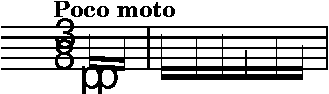
\includegraphics[width=0.7\linewidth]{fur_elise.pdf}
\end{frame}

\begin{frame}\frametitle{}
  \centering
  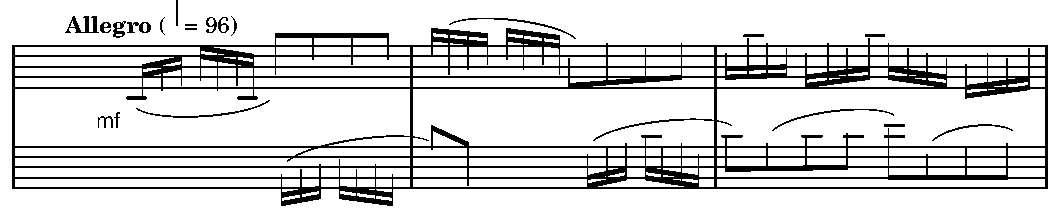
\includegraphics[width=\linewidth]{invention1.pdf}
\end{frame}

\end{document}
